\begin{frame}
\frametitle{About This Work...}

\emph{A Graph Model for False Negative Handling in Indoor RFID Tracking Data}.~\cite{baba2013graph}\\
A.I.~Baba, H.~Lu, T.B.~Pedersen, X.~Xie\\~\\

\emph{Handling False Negatives in Indoor RFID Data}.~\cite{baba2014handling} \\
A.I.~Baba, H.~Lu, T.B.~Pedersen, X.~Xie\\~\\

\begin{itemize}
  \item Published at \emph{SIGSPAITAL' 2013}, \emph{MDM' 2014}.
  \item Focuses on handling \emph{false negatives} which occur when a moving object passes the detection range of an RFID reader but the reader fails to produce any readings.
  \item Proposes the transition probabilities that capture how likely objects move from one RFID reader to another.
\end{itemize}

\end{frame}

%------------------------------------------------

\begin{frame}
\frametitle{Motivation}

\begin{itemize}
  \item RFID emerges to be one of the key technologies to modernize object tracking and monitoring systems in indoor environments.
  \begin{sitemize}
    \item airport baggage tracking
  \end{sitemize}
  \item However, the unreliable nature of raw data captured by readers is a major factor hindering the development of various applications.
  \begin{sitemize}
    \item loss and error rate can be between 30-40\%.~\cite{floerkemeier2004issues}
    \item read events are frequently missed due to the detection ability of a reader, the quality of an RFID tag, and constraints of the environment.~\cite{derakhshan2007rfid}
  \end{sitemize}
  \item Critical to cleanse the RFID raw data, and provide clean data to high level applications to make correct interpretations and analysis of the physical world.
\end{itemize}

\end{frame}

%------------------------------------------------

\begin{frame}
\frametitle{False Negatives}

\begin{figure}[tb]
  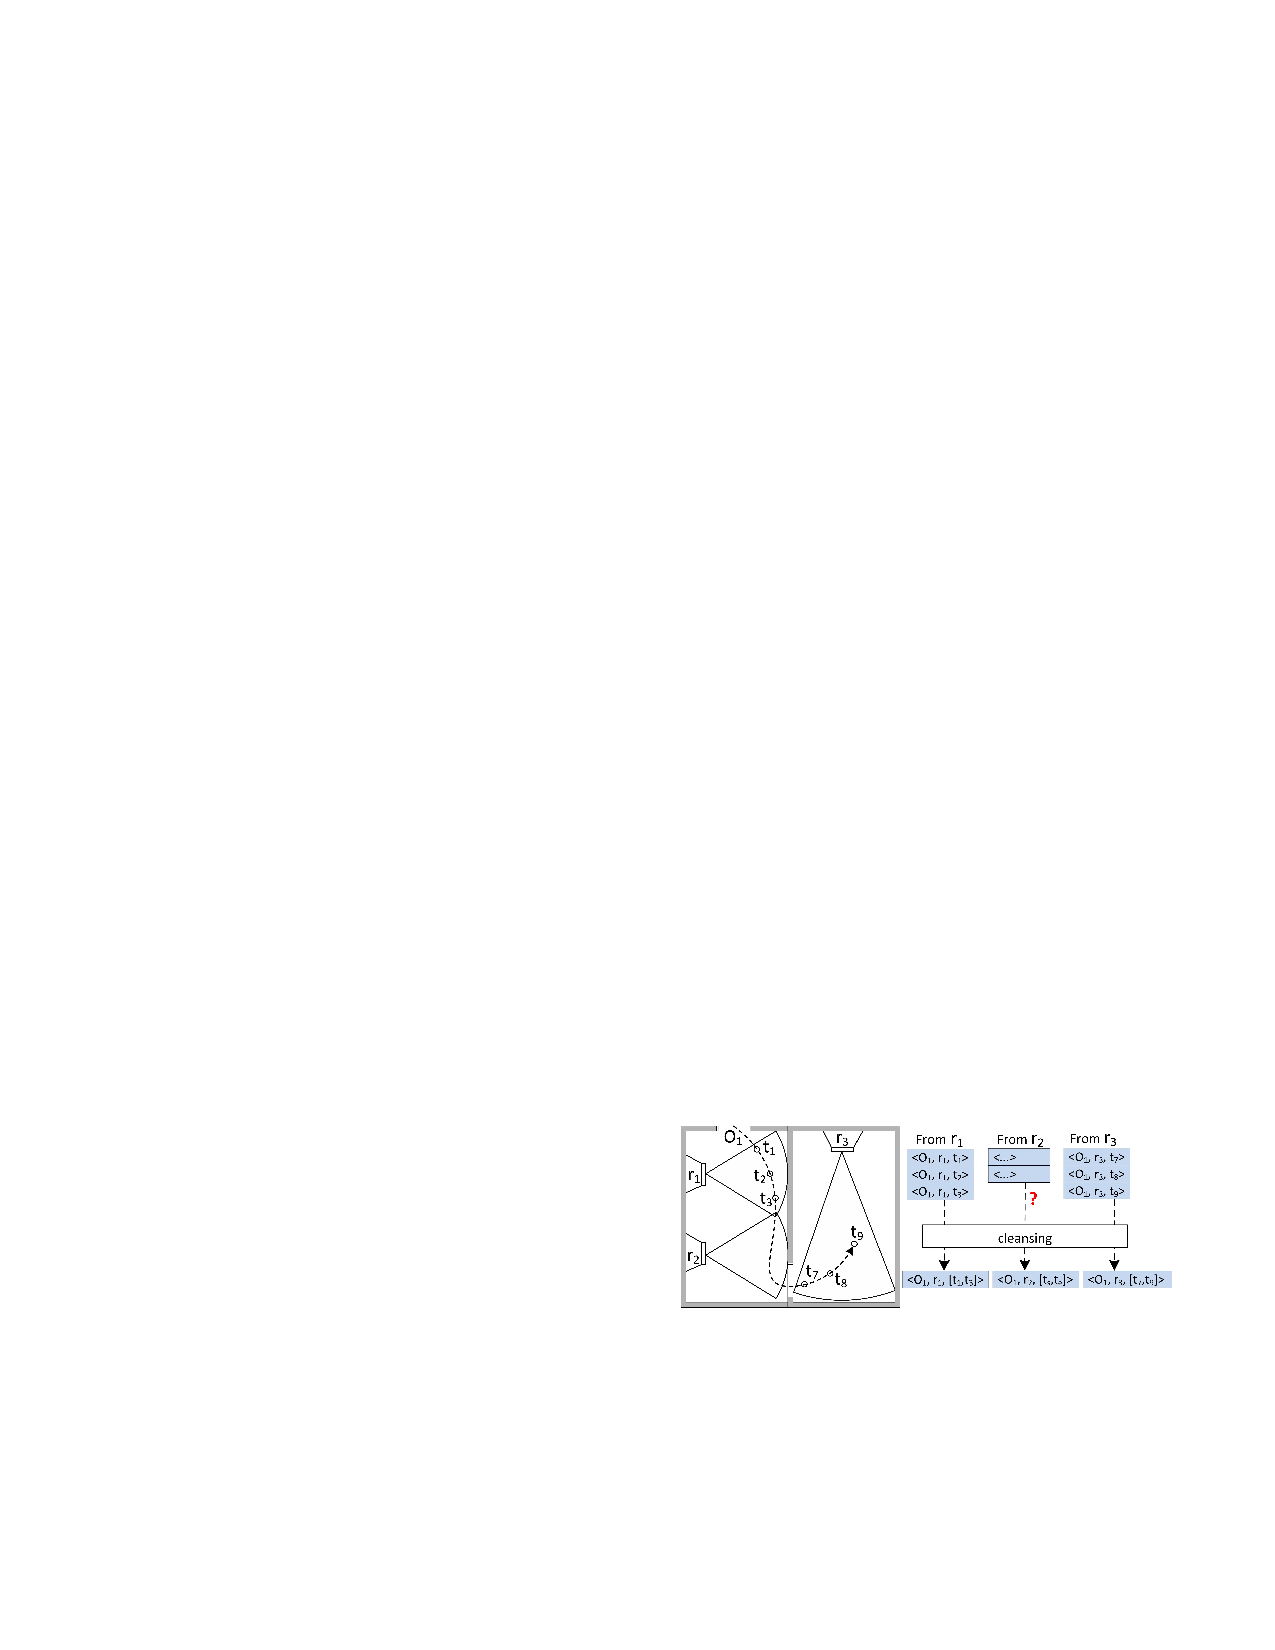
\includegraphics[width=0.8\columnwidth]{figures/3-3/3-3-1.pdf}
\end{figure}
\vspace{-10pt}
\begin{example}
  \ssize{
  two readers $r_1$ and $r_2$ in one hall and $r_3$ in another hall. Object $O_1$ enters the hall at time $t_1$ and is continuously tracked by $r_1$ until $t_3$. After that, $O_1$ is detected by $r_3$ at $t_7$ and $r_3$ keeps tracking $O_1$ until $t_9$. However, $O_1$ is not supposed to be detected by $r_3$ before it's detected by reader $r_2$ on its way, because to enter into the hall where $r_3$ is, $O_1$ must pass the detection range of $r_1$ and $r_2$ and cannot remain undetected for time interval $[t_3, t_7]$.
  }
\end{example}

\end{frame}

%------------------------------------------------

\begin{frame}
\frametitle{Aggregate Tracking Table (ATT)~\cite{baba2013spatiotemporal}}

\begin{itemize}

  \item All raw readings are ordered by their detection times and are aggregated into tracking records in \conceptbf{Aggregate Tracking Table}($ATT$).

  \item Each generated tracking record is in the format of $(deviceID, objectID, t_s, t_e, r_{Count})$.

  \item The meaning is that object identified by $objectID$ is detected by device identified by $deviceID$ during time interval $[t_s, t_e]$ for $r_{Count}$ times.
\end{itemize}

\end{frame}

%------------------------------------------------

\begin{frame}
\frametitle{Definitions}

\begin{definition}[False Negatives]
  Given a reader $r_i$ and a moving object $O$, if object $O$ goes through the detection range of reader $r_i$ during time interval $[t, t']$, but $r_i$ does not generate any reading about $O$'s presence during time interval $[t, t']$, a false negative occurs in the data.
\end{definition}

\begin{definition}[False Negatives Handling]
  Given an $ATT$, the false negative handling process detects false negatives and inserts recovered tracking records into the $ATT$.
\end{definition}

\end{frame}

%------------------------------------------------

\begin{frame}
\frametitle{Transition Probabilities}

\conceptbf{Markov Property}: each step a move to next reader (vertice) only depends on current reader and not the readers that precede it, holding a ``memorylessness''.\\~\\ \pause

A moving object at reader $r_i$ moves to a neighboring reader $r_j$ with a probability proportional to the probability weight of the edge $(r_i, r_j)$, i.e., the probability of a transition from $r_i$ to neighboring $r_j$ is : \pause
\begin{equation}
  \frac{p(r_i, p_j)}{\sum_{k \in N(r_i)}p(r_i, K)}
\end{equation}

\pause
Here, $N(r_i)$ is the set of neighbors of reader $r_i$. The transitional probability $p(r_i, r_j)$ denotes the probability that a moving object is detected by $r_j$ at some time later after $t$ given that it was detected by $r_i$ at time $t$ without any third reader involved in-between.

\end{frame}

%------------------------------------------------

\begin{frame}
\frametitle{Transition Probabilities}

\begin{definition}[Transition]
  A transition takes place when a moving object moves from a reader $r_i$ to another reader $r_j$ without passing through any intermediate readers.
\end{definition}

\vspace{10pt}

\conceptbf{A transition probability matrix} represents the transition relationship between a finite number of readers:
\begin{equation}
  P = \begin{bmatrix}
p(r_1, r_1) & p(r_1, r_2) & \cdots & p(r_1, r_n)\\
p(r_2, r_1) & p(r_2, r_2) & \cdots & p(r_2, r_n)\\
\vdots & \vdots & \vdots & \vdots\\
p(r_n, r_1) & p(r_n, r_2) & \cdots & p(r_n, r_n)
\end{bmatrix}
\end{equation}

\vspace{5pt}

For each deployed reader $r_i$, $\sum_{j=1}^{n}p(p_i,p_j) = 1$.

\end{frame}

%------------------------------------------------

\begin{frame}
\frametitle{Transition Probabilities}

The elements of the transition matrix $P$ are then obtained as follows:

\vspace{10pt}

\begin{equation}
  p(r_i, p_j) = \left\{\begin{matrix}
\frac{N_{ij}}{N_i} & \text{if}~(r_i, r_j) \in G_{pdm}.E\\
0 & \text{otherwise}
\end{matrix}\right.
\end{equation}

\vspace{10pt}

where $N_{ij}$ is the number of objects moving from $r_i$ to $r_j$, $N_i$ is the total number of objects moving from $r_i$, $G_{pdm}$ is a probabilistic distance-aware graph model.

\end{frame}

%------------------------------------------------

\begin{frame}
\frametitle{Probabilistic Distance-Aware Graph Model}

\begin{block}{Probabilistic Distance-Aware Graph Model}
  $G_{pdm} = (V, E, \mathcal{L}_V, \mathcal{L}_E)$
  \begin{fitemize}
    \item $V$ is a set of vertices, each represents a deployed device $r_i$.
    \item $E$ is the set of edges, where $E = \{ (r_i, r_j) | r_i, r _j \in V \cup r_i \neq r_j \}$, one can move from $r_i$ to $r_j$ without being detected by third reader.
    \item $\mathcal{L}_V: V \rightarrow \mathcal{R} \times \mathcal{R}$ assigns to a vertex $v_i$ a minimum dwell time and sampling frequency of a corresponding reader $r_i$, i.e., $mathcal{L}_V(r_i) = (d_t, S_f)$.
    \item $\mathcal{L}_E: E \rightarrow \mathcal{R} \times \mathcal{R}$ assigns to an edge $(r_i, r_j)$ the minimum indoor walking time between two devices $r_i$ and $r_j$ and the probability with which an object can move between them, i.e., $mathcal{L}_E(r_i, r_j) = (t_{i,j}, p_{r_i,r_j})$.
  \end{fitemize}
\end{block}

\end{frame}

%------------------------------------------------

\begin{frame}
\frametitle{Probabilistic Distance-Aware Graph Model}

\begin{columns}

  \column{0.6\textwidth}
  \begin{figure}[tb]
    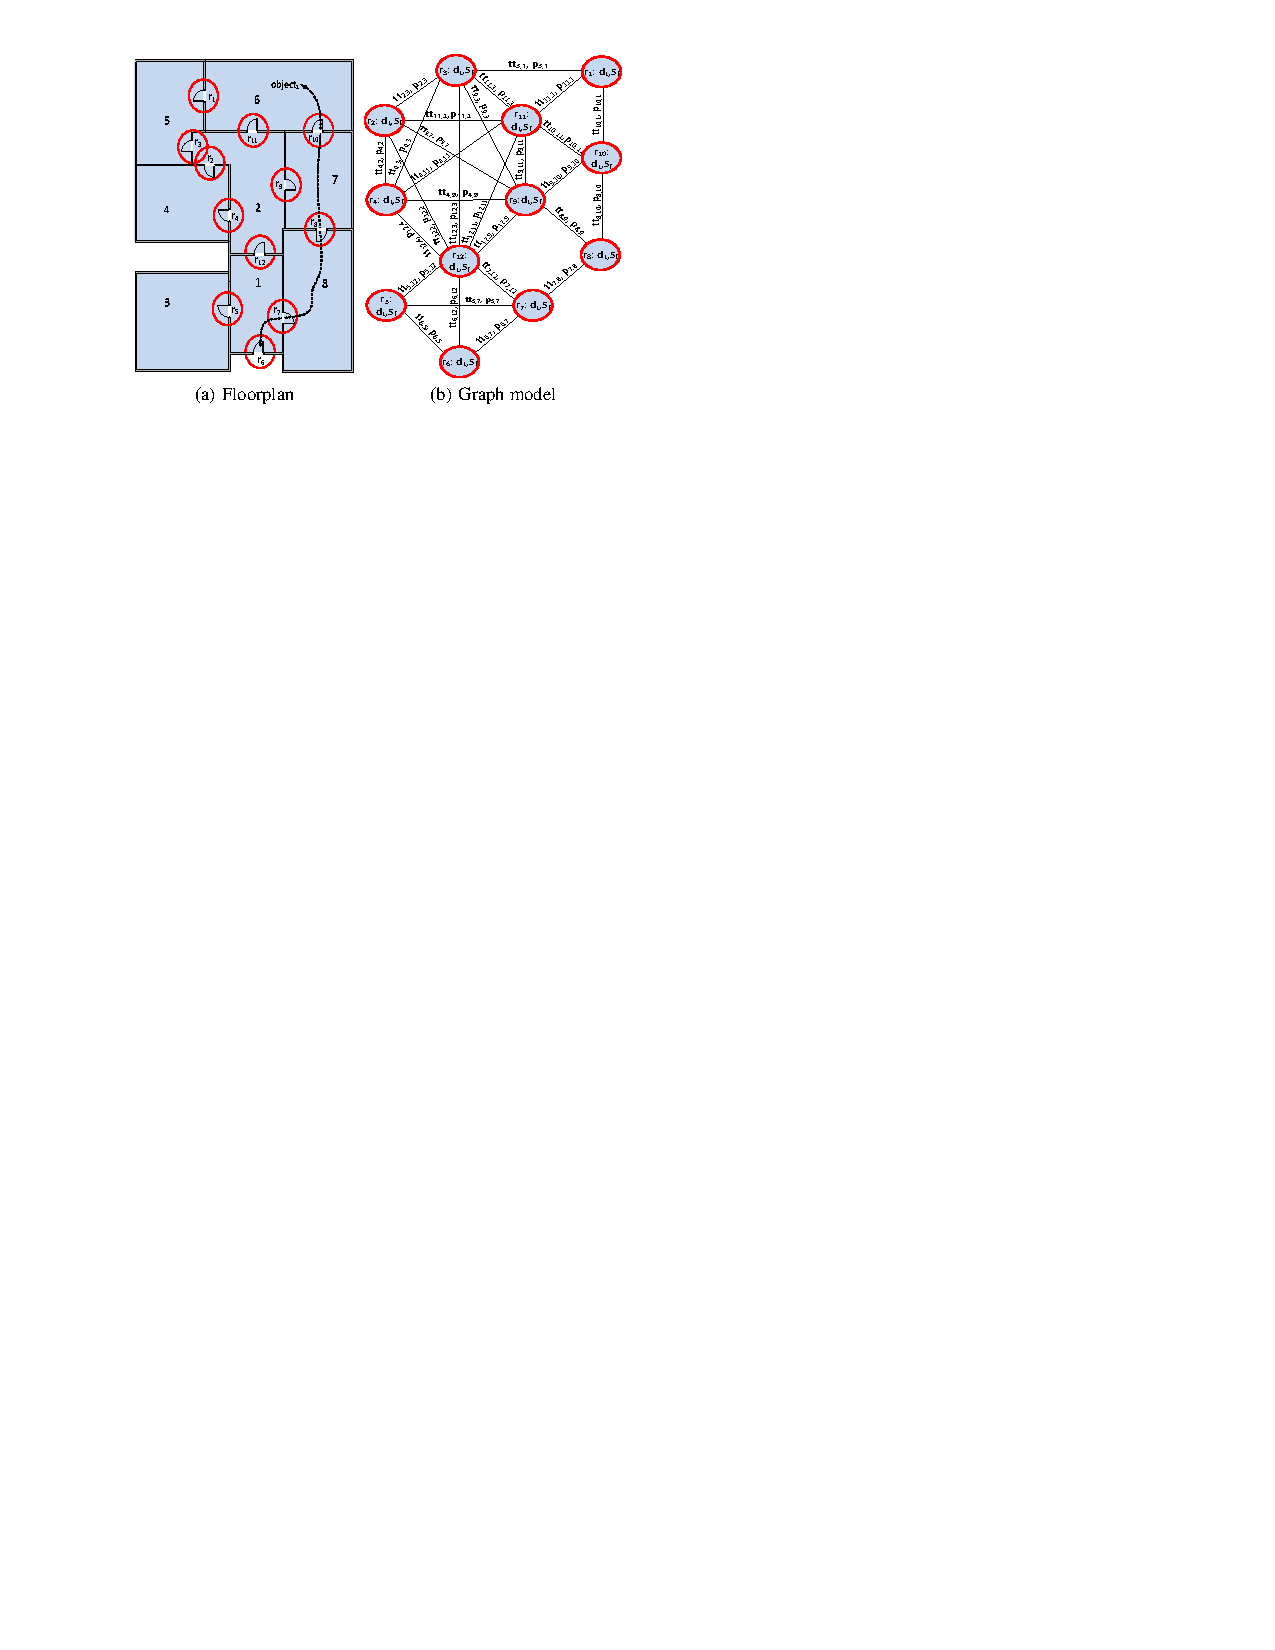
\includegraphics[width=\columnwidth]{figures/3-3/3-3-2.pdf}
  \end{figure}

  \column{0.4\textwidth}
  \begin{fitemize}
    \item the graph is enhanced from a distance deployment graph proposed in \cite{baba2013spatiotemporal}.
    \item different readers usually imply different minimum dwell times for detection and different sampling rates.
    \item the probability weight between two readers will be used to predict the most likely path an object may have taken.
  \end{fitemize}

\end{columns}

\end{frame}

%------------------------------------------------

\begin{frame}
\frametitle{Probabilistic Distance-Aware Graph Construction}

\begin{columns}

  \column{0.55\textwidth}
  \begin{figure}[tb]
    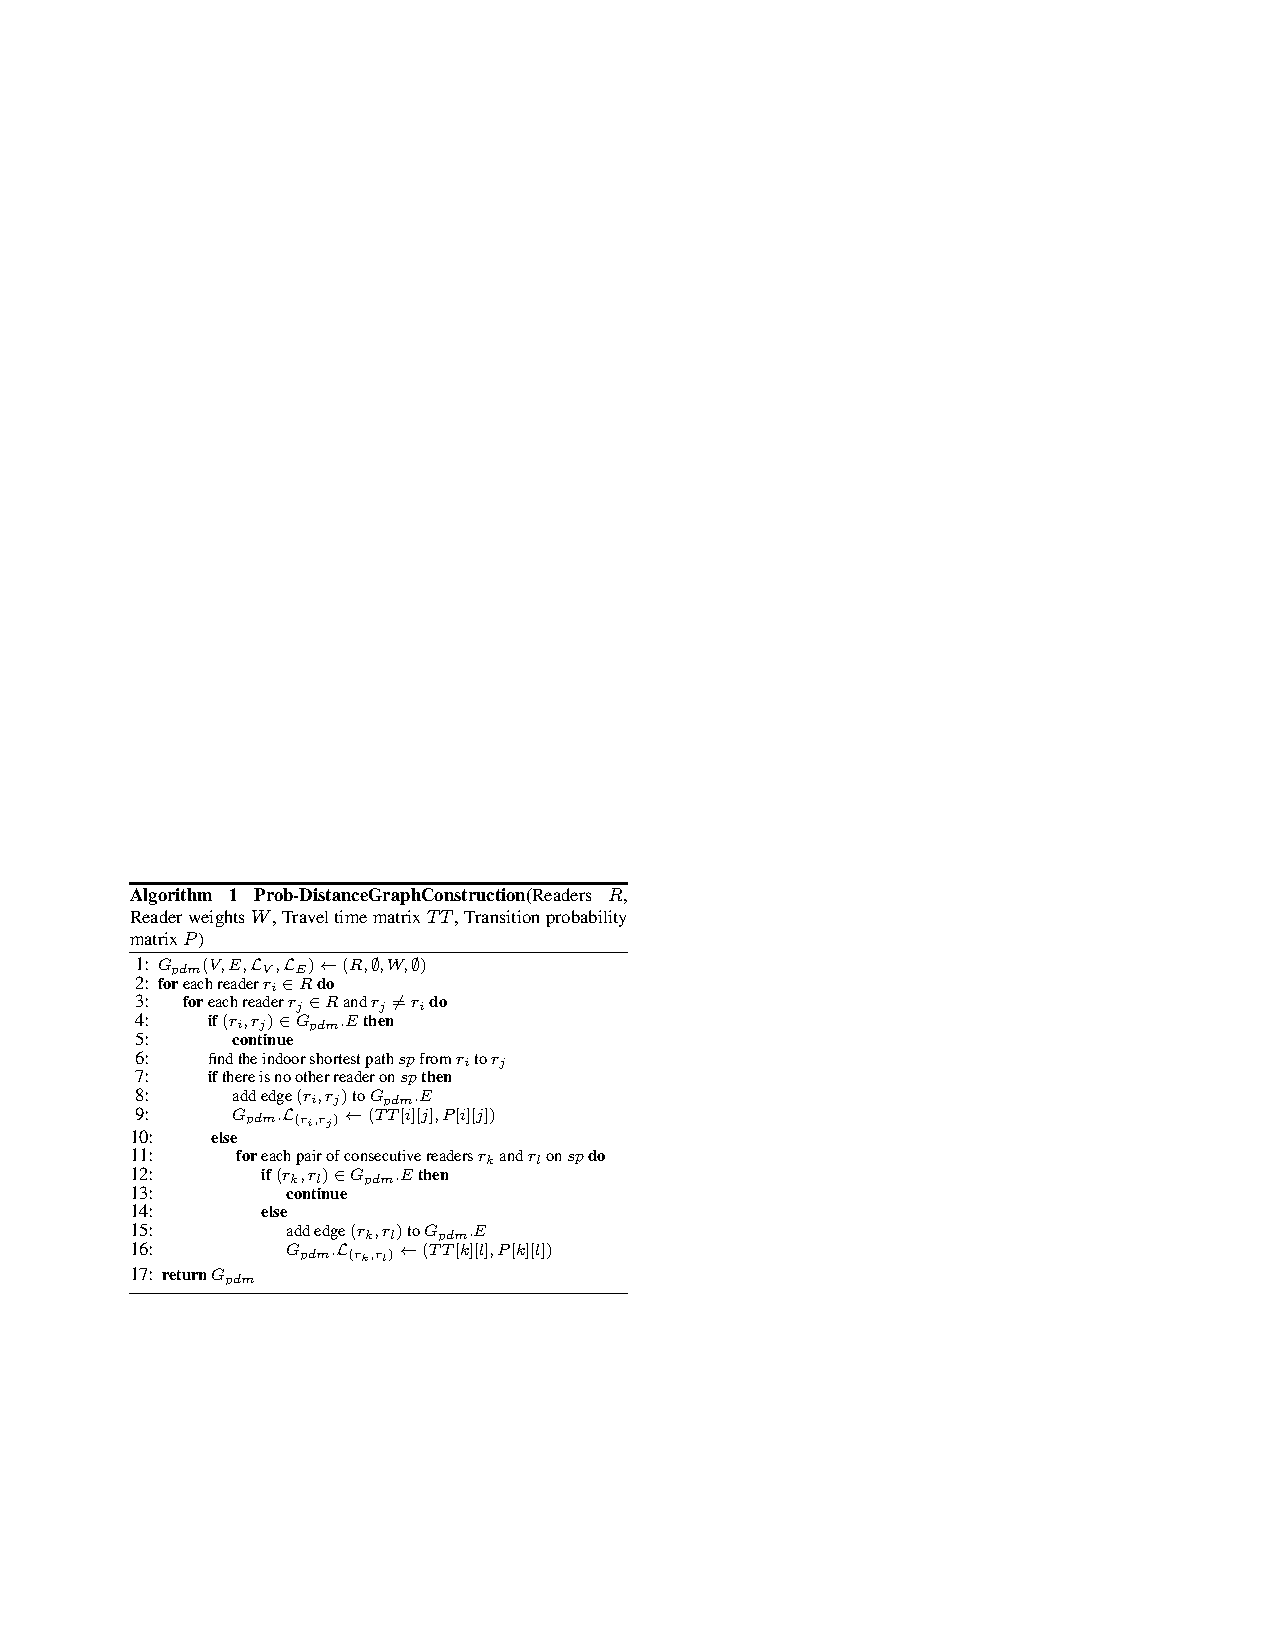
\includegraphics[width=\columnwidth]{figures/3-3/3-3-3.pdf}
  \end{figure}

  \column{0.45\textwidth}
  \begin{enumerate}
    \ssize{
    \item lines 2--6: the indoor shortest path $sp$ is found if the edge $(r_i, r_j)$ is not in the graph yet.
    \item lines 7--9: if $sp$ only contains readers $r_i$ and $r_j$, a new edge is created with the corresponding weights.
    \item lines 11-16: otherwise, each pair of consecutive readers on $sp$ are processed likewise.
    \item indoor shortest paths are computed according to the algorithms in \cite{DBLP:conf/icde/LuCJ12}.
    }
  \end{enumerate}

\end{columns}

\end{frame}

%------------------------------------------------

\begin{frame}
\frametitle{Handling False Negatives}

\begin{definition}[Path]
  A path is a sequence of readers $r_1, r_2, ..., r_n$ where there is an edge connecting $r_i$ and $r_{r+1}$ for $i = 1, 2,...,n$. A path is simple if all $r_i$ are distinct.
\end{definition}

\begin{definition}[Candidate Path]
  Given a source reader $R_s$ and a destination reader $R_d$, a path from $R_s$ to $R_d$, represented as $R_s \overset{\delta}{\rightsquigarrow} R_d$ is a candidate path, if a path $\delta$ satisfies the spatio-temporal constraints captured by a graph.
\end{definition}

\end{frame}

%------------------------------------------------

\begin{frame}
\frametitle{Handling False Negatives}

\begin{definition}[Most Likely Path]
  Given a set of candidate path $\{ \delta_m \}_{m=1}^n$, a most likely path is:
  \begin{equation}
    \delta^* = {\arg\max}_m \prod_{E_{ij} \in \delta_m} p_{i,j}
  \end{equation}
\end{definition}

A two-phase solution is designed to handle false negatives in indoor tracking data, \emph{detecting false negatives} and \emph{recovering false negatives}.

\end{frame}

%------------------------------------------------

\begin{frame}
\frametitle{Topological Scenarios I}

\begin{figure}[tb]
  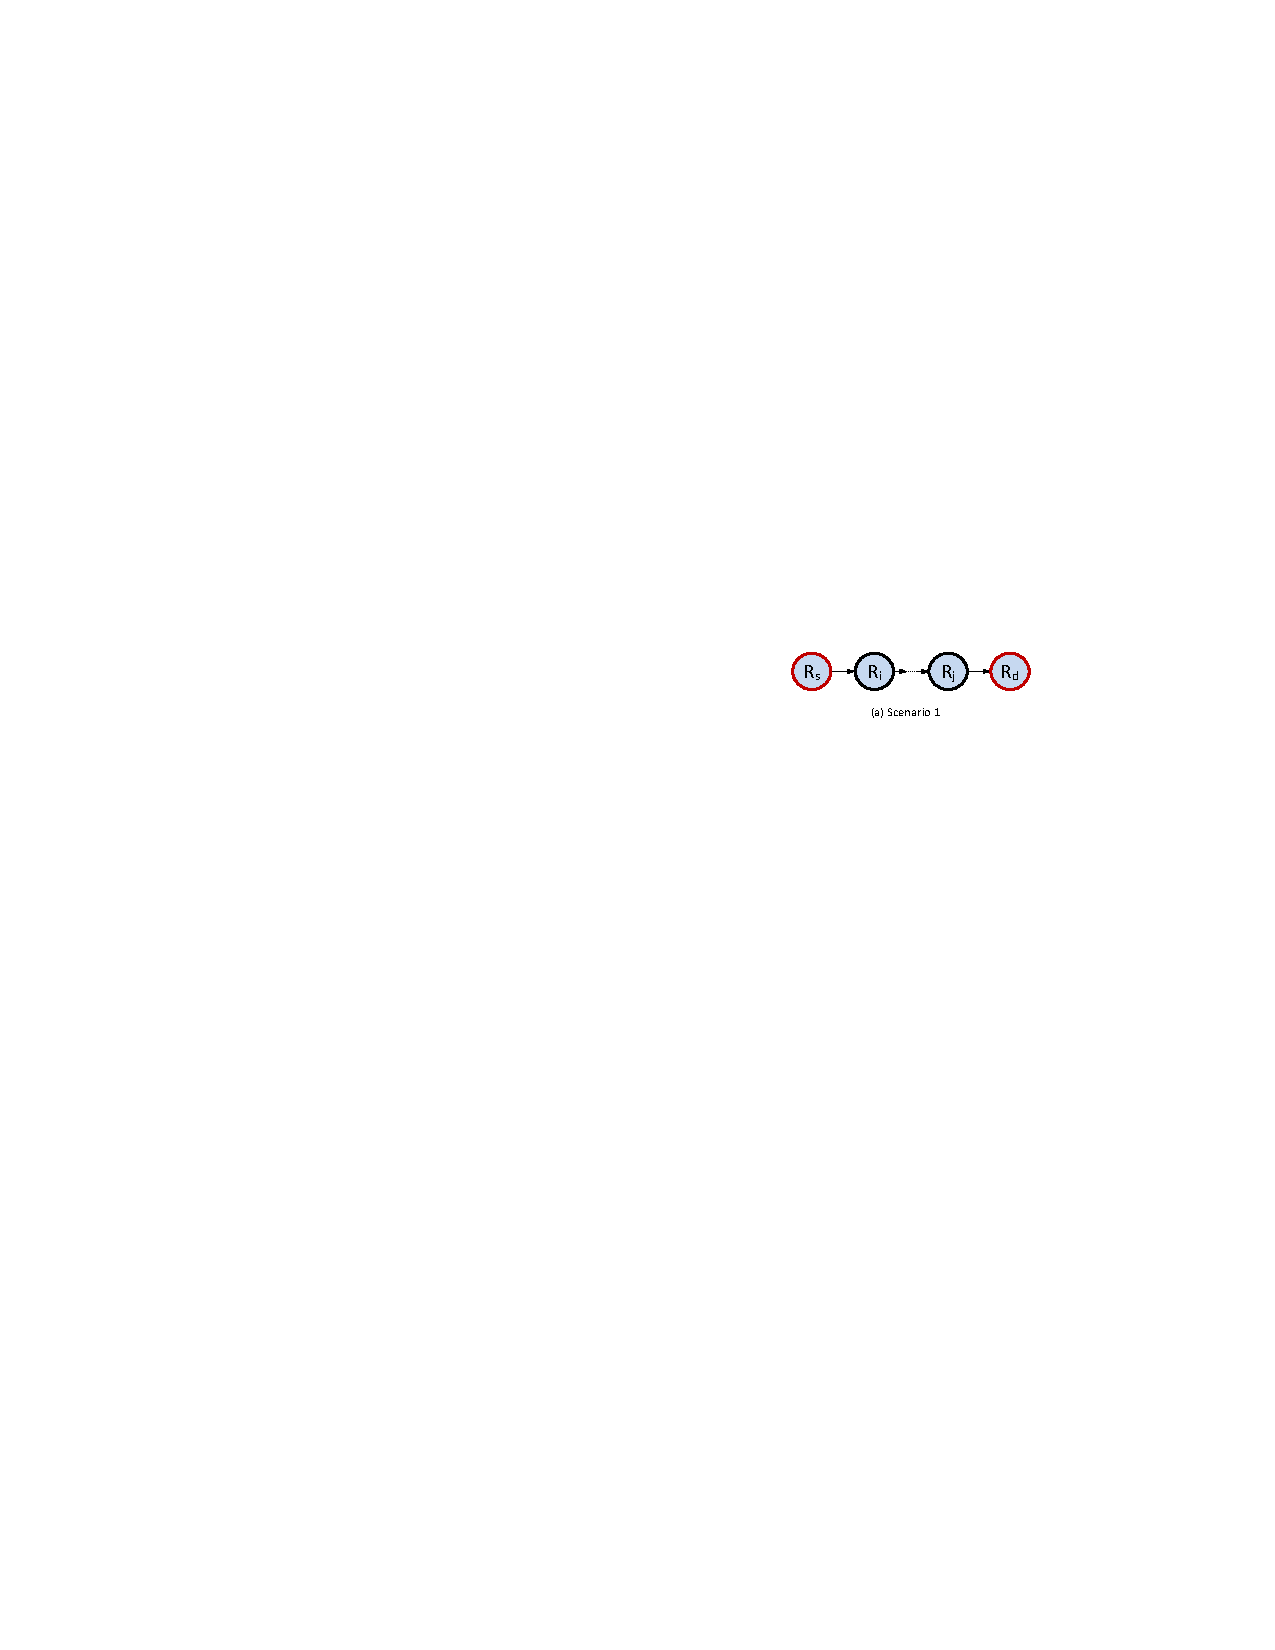
\includegraphics[width=0.8\columnwidth]{figures/3-3/3-3-4.pdf}
\end{figure}

a sigle path from source reader $R_s$ goes to a destination reader $R_d$. Between $R_i$ and $R_j$ there can be none or many readers deployed all connected in linear fashion.

\end{frame}

%------------------------------------------------

\begin{frame}
\frametitle{Topological Scenarios II}

\begin{figure}[tb]
  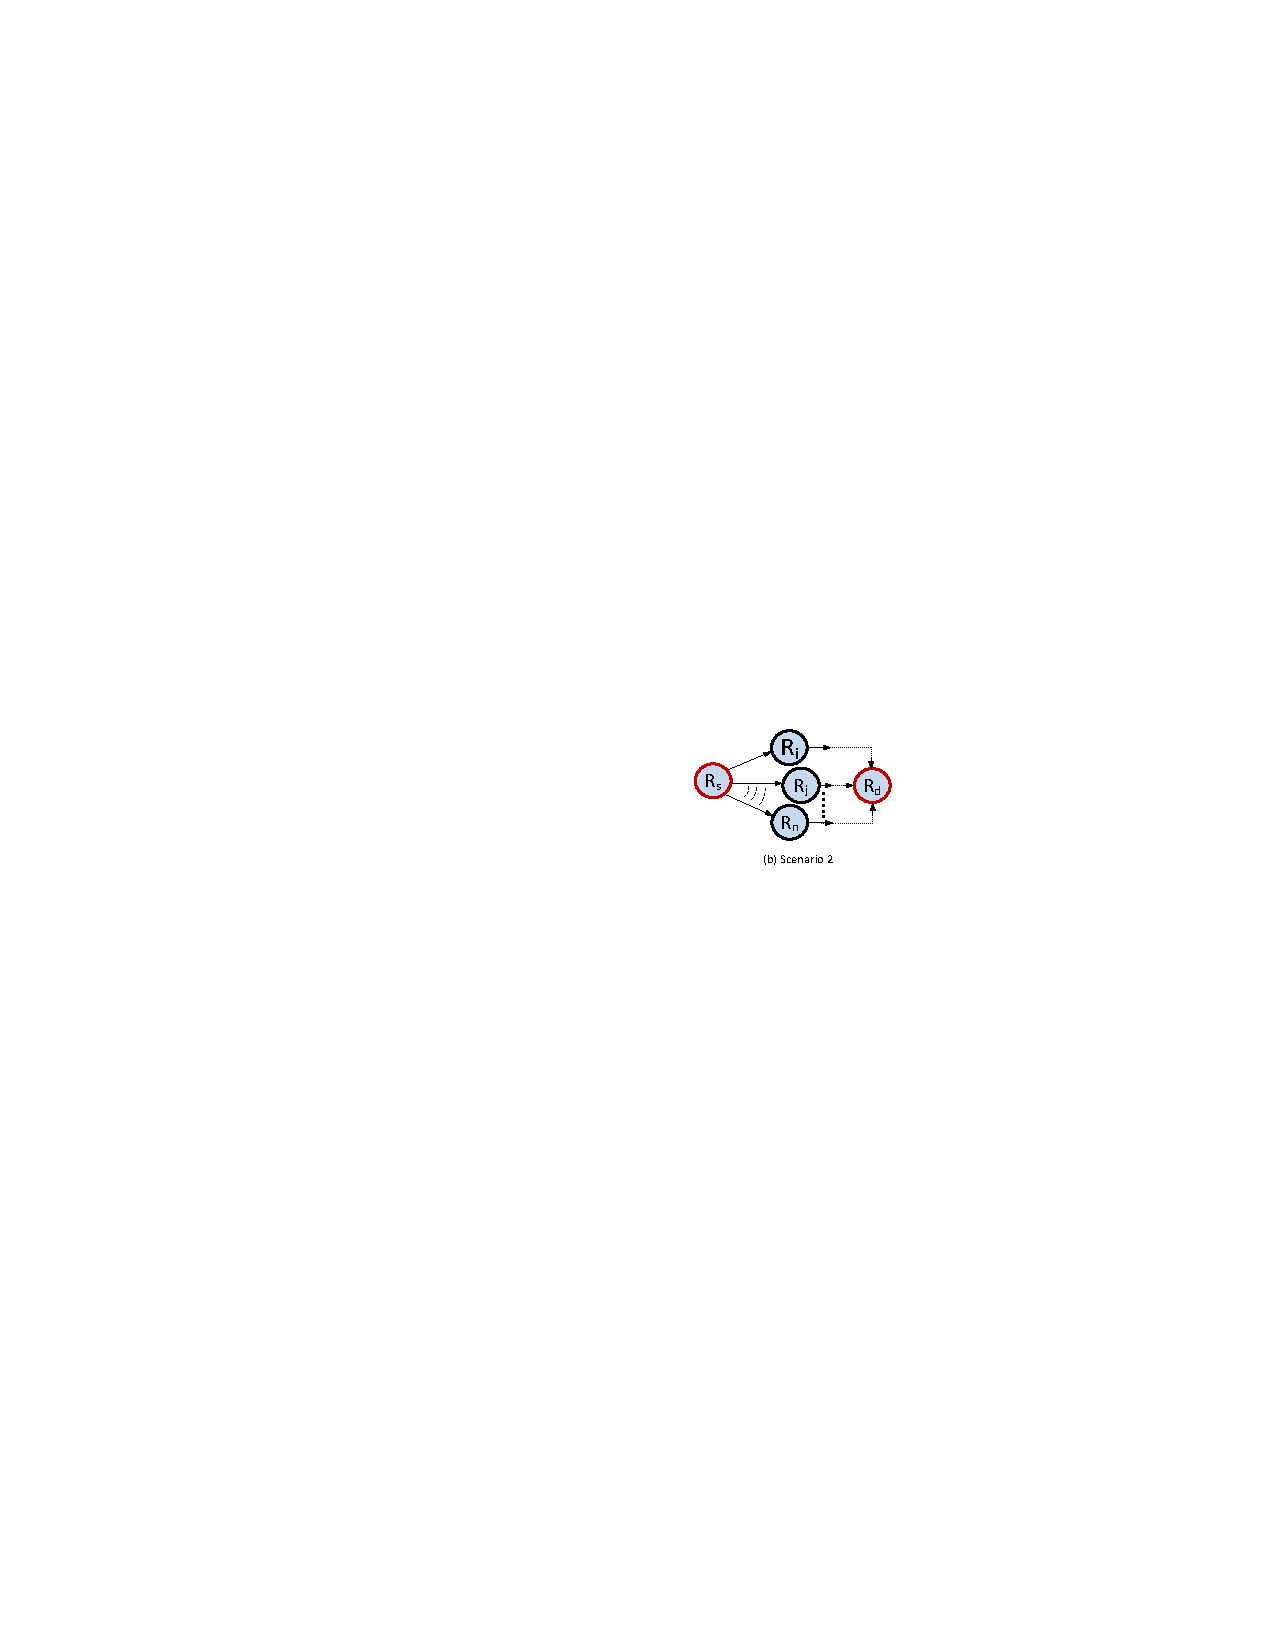
\includegraphics[width=0.6\columnwidth]{figures/3-3/3-3-5.pdf}
\end{figure}
\vspace{-10pt}
Source reader $R_s$ have many outgoing edges to $R_i$, $R_j$ to $R_n$. Once the candidates paths are found, transitions probabilities captured by each edge of graph can be used to choose the most probable path to reach destination reader $R_d$.

\end{frame}

%------------------------------------------------

\begin{frame}
\frametitle{Topological Scenarios III}

\begin{figure}[tb]
  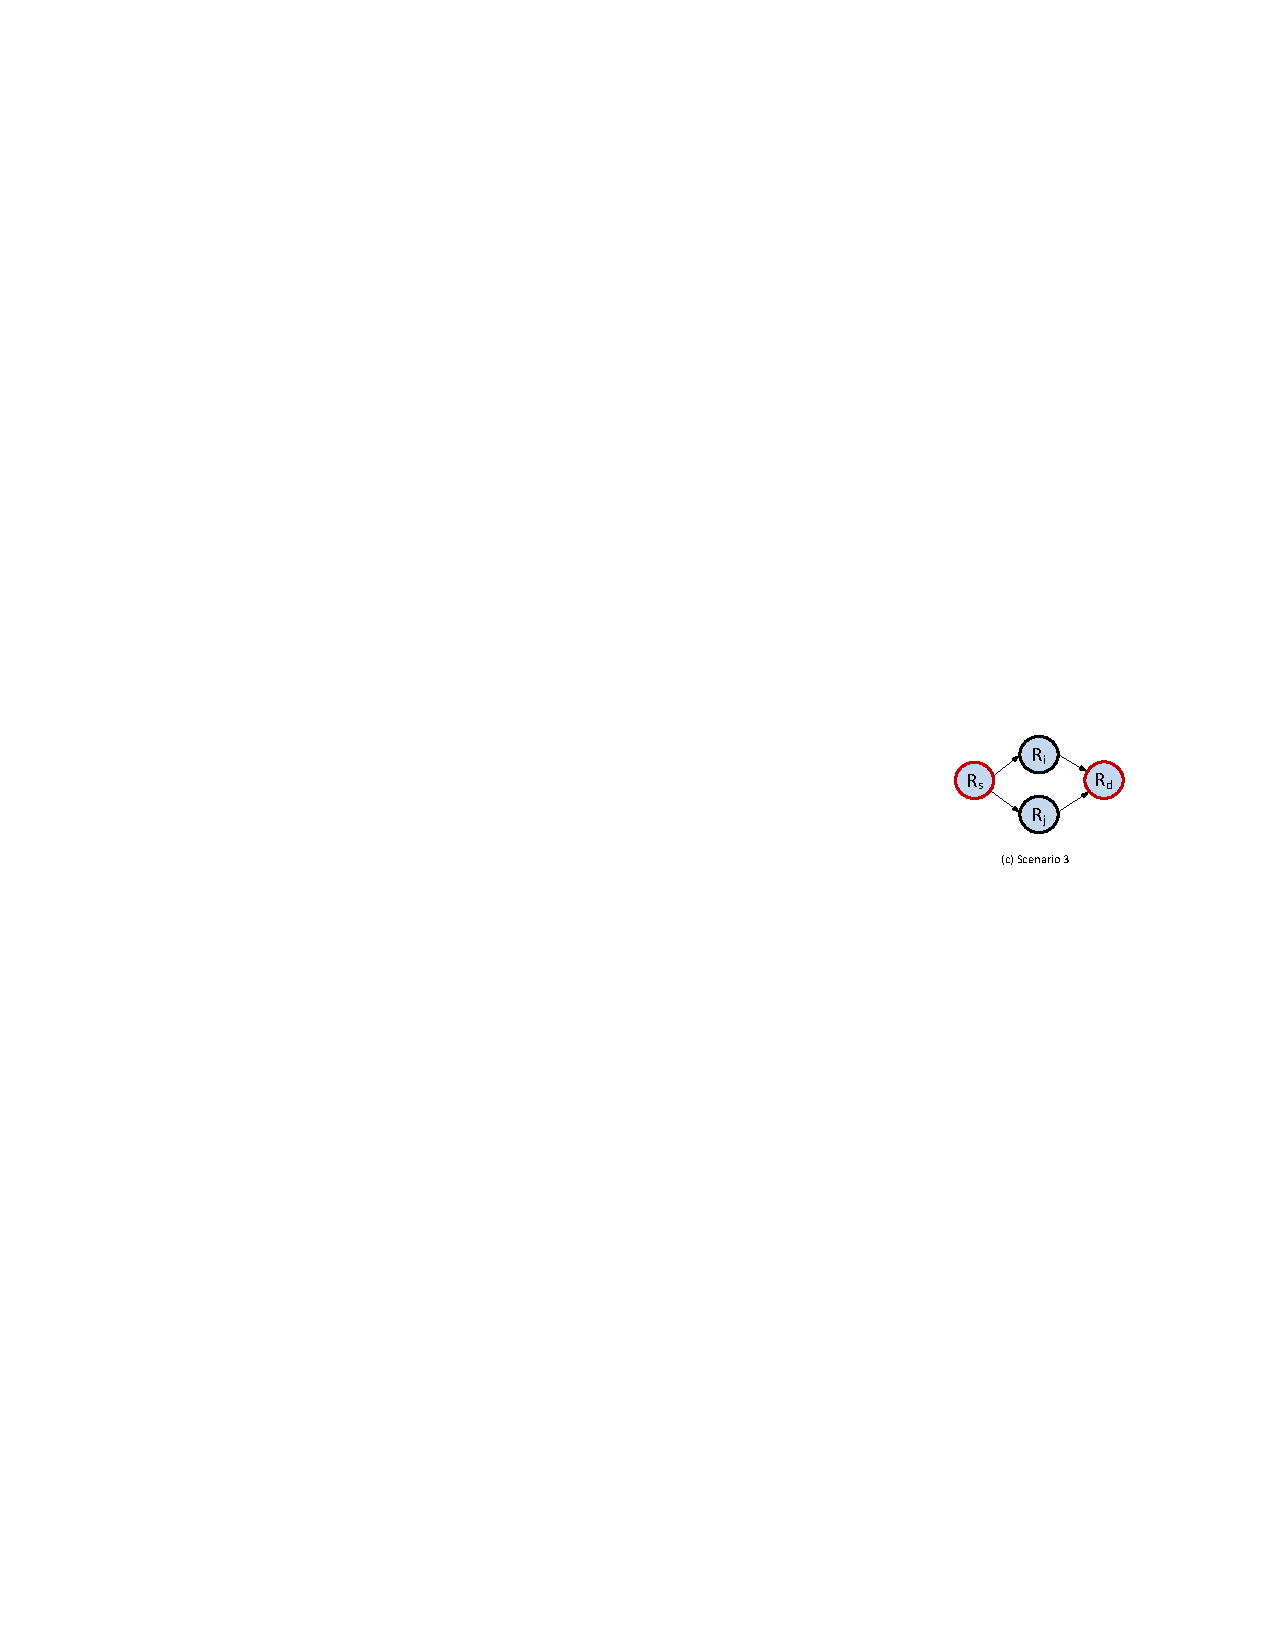
\includegraphics[width=0.55\columnwidth]{figures/3-3/3-3-6.pdf}
\end{figure}
\vspace{-10pt}
A sub-case of previous case. Both paths satisfies the spatio-temporal constraints equally, making it difficult to directly find a first candidate path. A most likely path will finally be decided on the transition probablities.

\end{frame}

%------------------------------------------------

\begin{frame}
\frametitle{Detecting False Negatives}

\begin{itemize}

  \item take aggregated tracking table $ATT$ as an input, identifies possible false negatives using the probabilistic distance-aware graph model of all deployed readers.

  \item look at each tracking record $tr$ in $ATT$ and find out the neighbors of $tr.deviceID$.

  \item take next tracking record $tr'$ and check if $tr'.deviceID$ is in a list of neighbors of $tr.deviceID$.

  \item if none of neighbors matches, it can be concluded that one or more readers between the two devices have failed to detect a moving object with identity $tr.objectID$.

  \item find the path between the two devices using the above definitions.

\end{itemize}

\end{frame}

%------------------------------------------------

\begin{frame}
\frametitle{Detecting False Negatives: Algorithm}

\begin{columns}

  \column{0.5\textwidth}
  \begin{figure}[tb]
    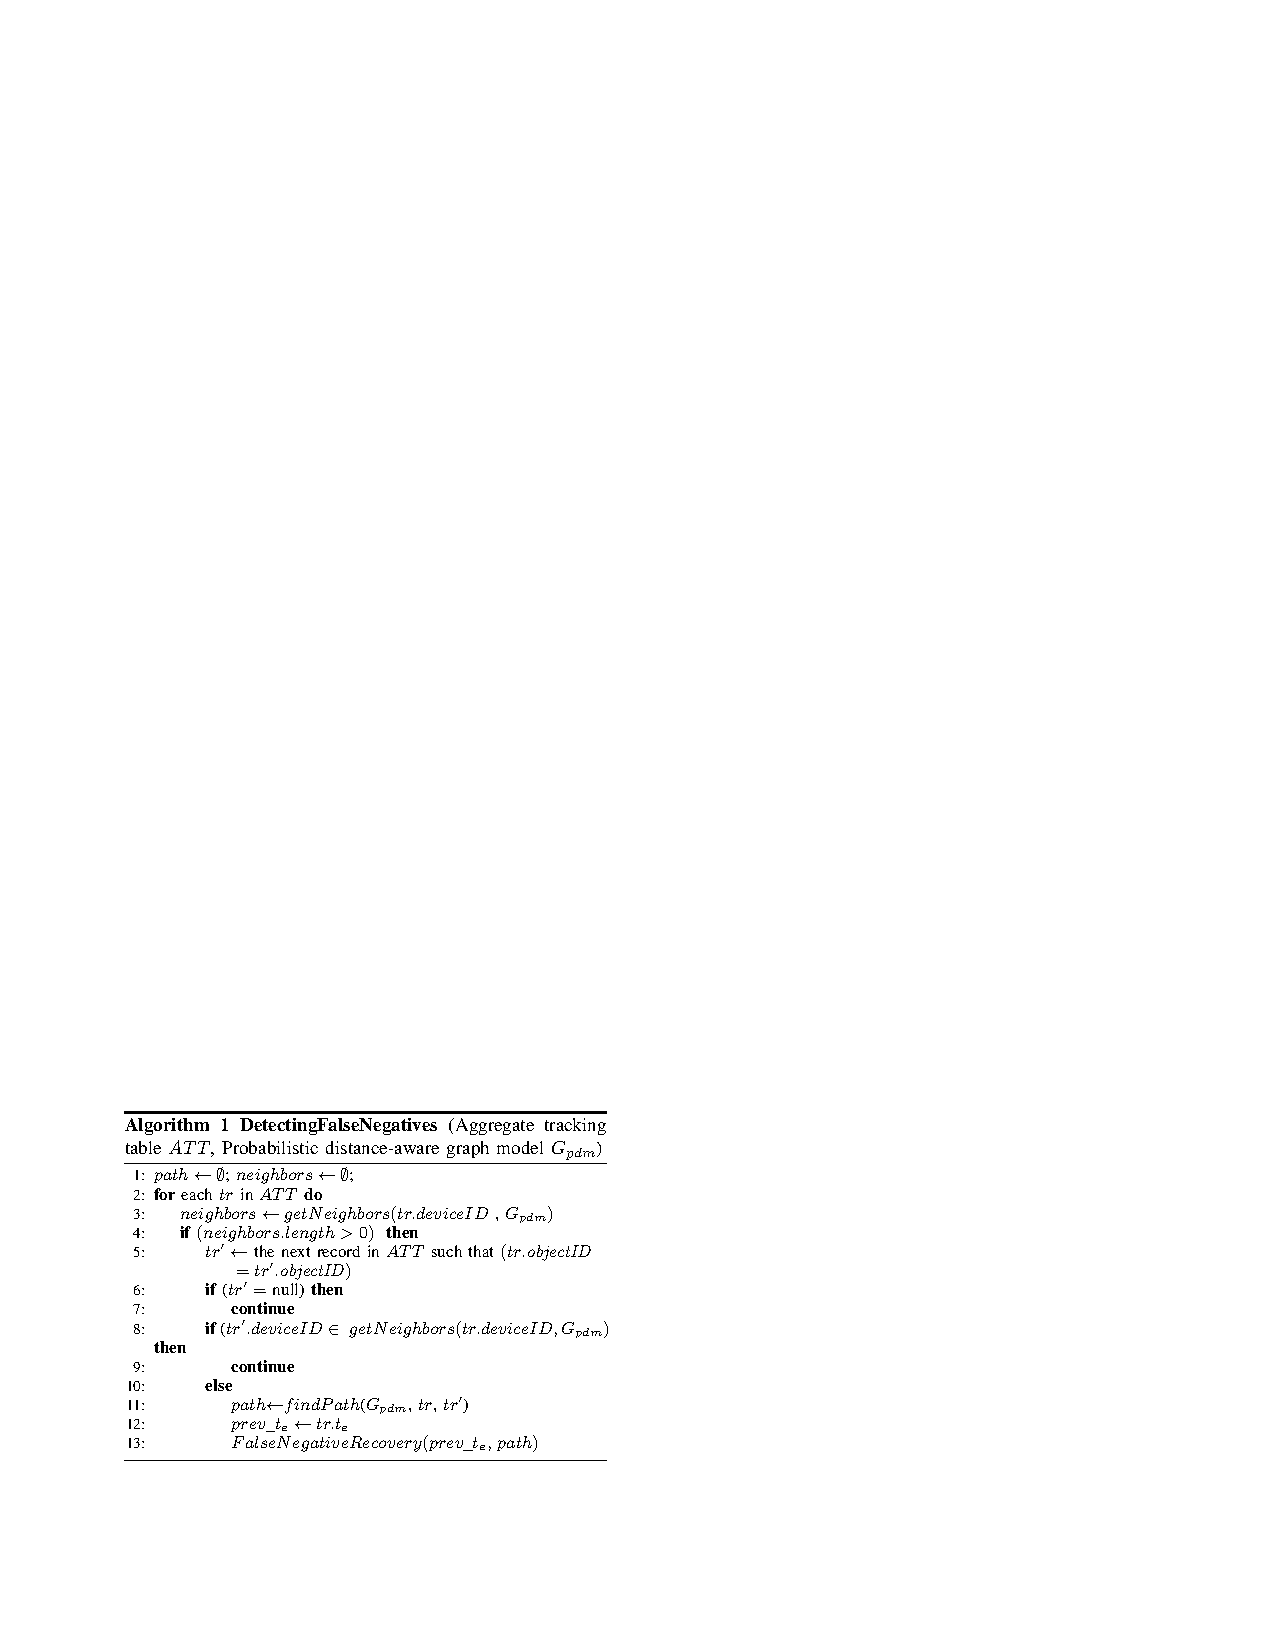
\includegraphics[width=\columnwidth]{figures/3-3/3-3-7.pdf}
  \end{figure}

  \column{0.5\textwidth}
  \begin{sitemize}
    \item line 3: find out all the outgoing neighbors of the first tracking device ($tr.deviceID$).
    \item line 4: check if the current device $tr.deviceID$ is not the last device
    \item lines 5--9: get $tr$'s next tracking record $tr'$ from $ATT$ that involves the same object as $tr$, if next tracking record is null, simply contunue with another object. If there is and $tr'.deviceID$ is equal to one of the neighbors, simply continue the process.
    \item lines 10-13: otherwise there is false negatives, call the function \emph{FalseNegativeRecovery}.
  \end{sitemize}

\end{columns}

\end{frame}

%------------------------------------------------

\begin{frame}
\frametitle{Algorithm: \emph{findAllPaths}}

\begin{columns}

  \column{0.5\textwidth}
  \begin{figure}[tb]
    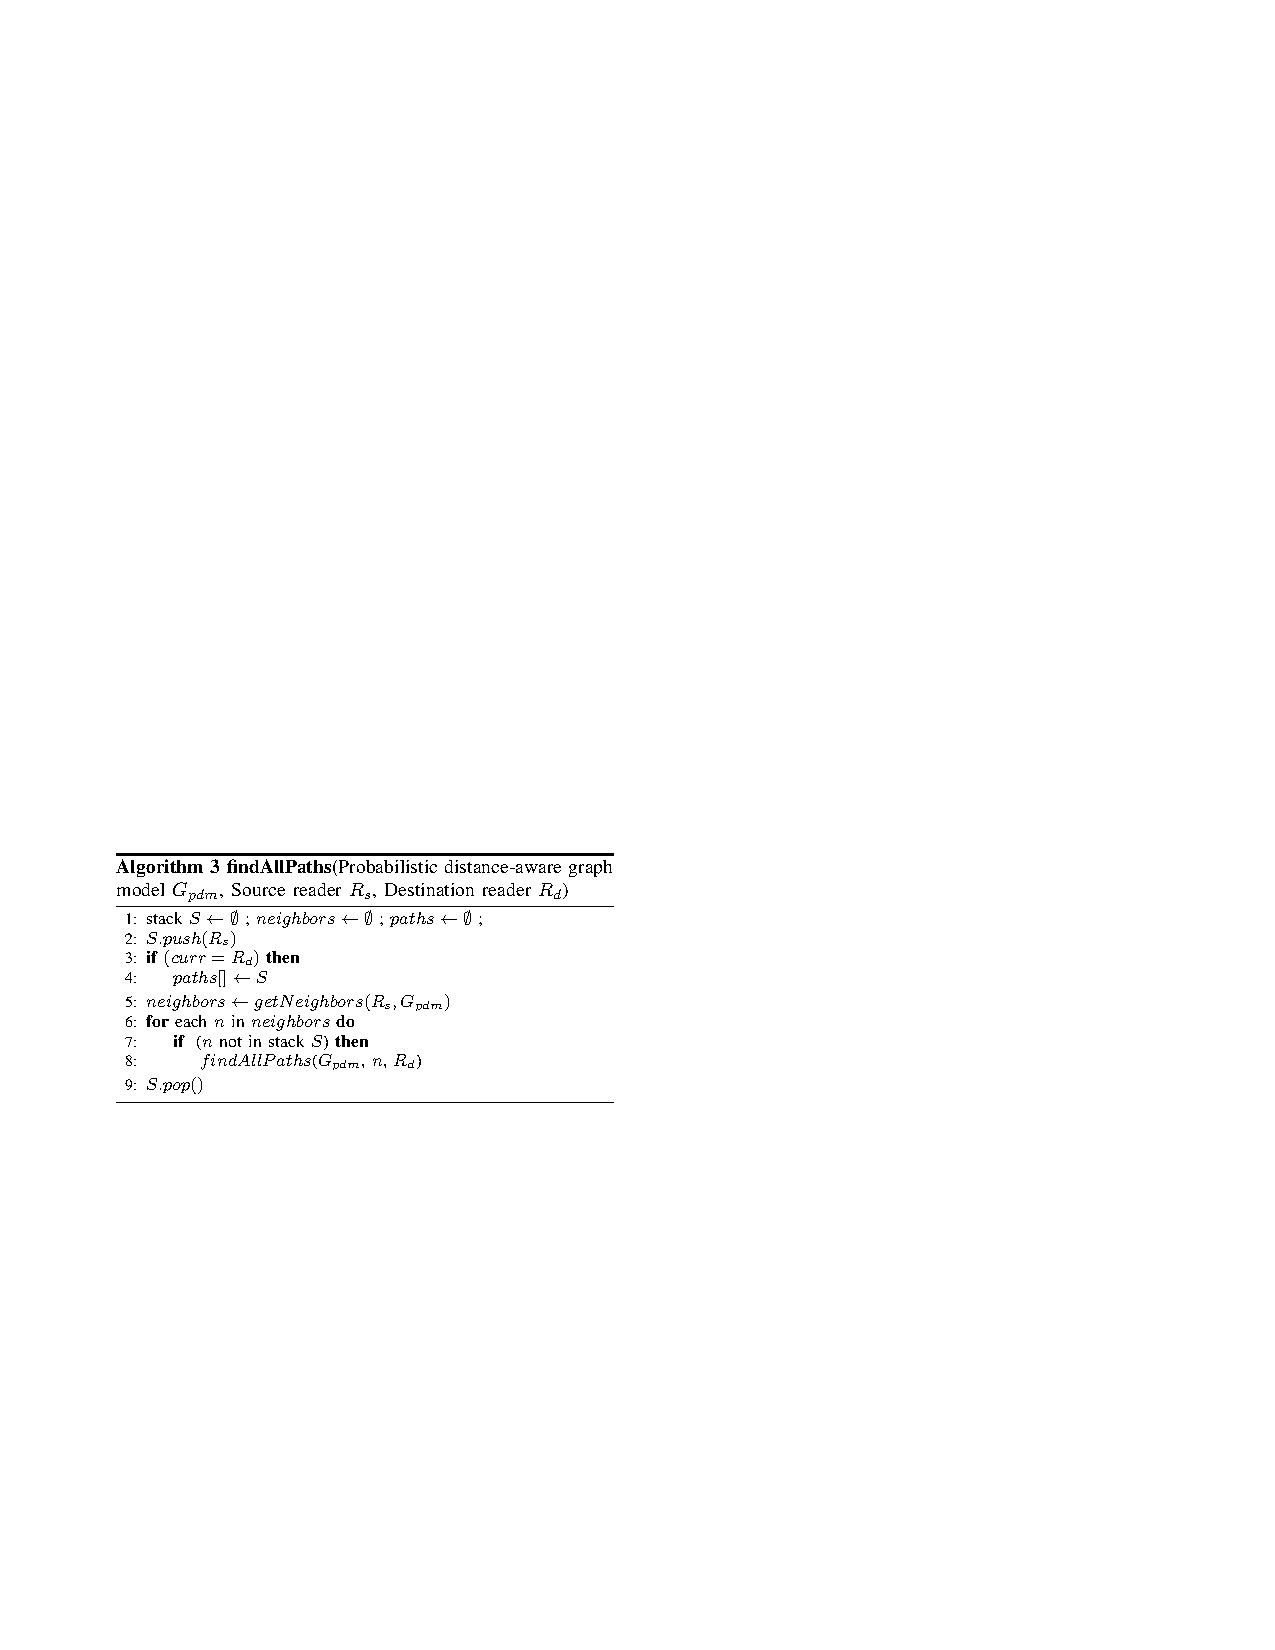
\includegraphics[width=\columnwidth]{figures/3-3/3-3-9.pdf}
  \end{figure}

  \column{0.5\textwidth}
  \begin{sitemize}
    \item takes a graph $G_{pdm}$, source reader $R_s$ and destination reader $R_d$ as input.
    \item returns all the paths between $R_s$ and $R_d$.
    \item follows an improved depth-first search paradigm, which estimates all the possible paths between two readers.
  \end{sitemize}

\end{columns}

\end{frame}

%------------------------------------------------

\begin{frame}
\frametitle{Algorithm: \emph{findPath}}

\begin{columns}

  \column{0.5\textwidth}
  \begin{figure}[tb]
    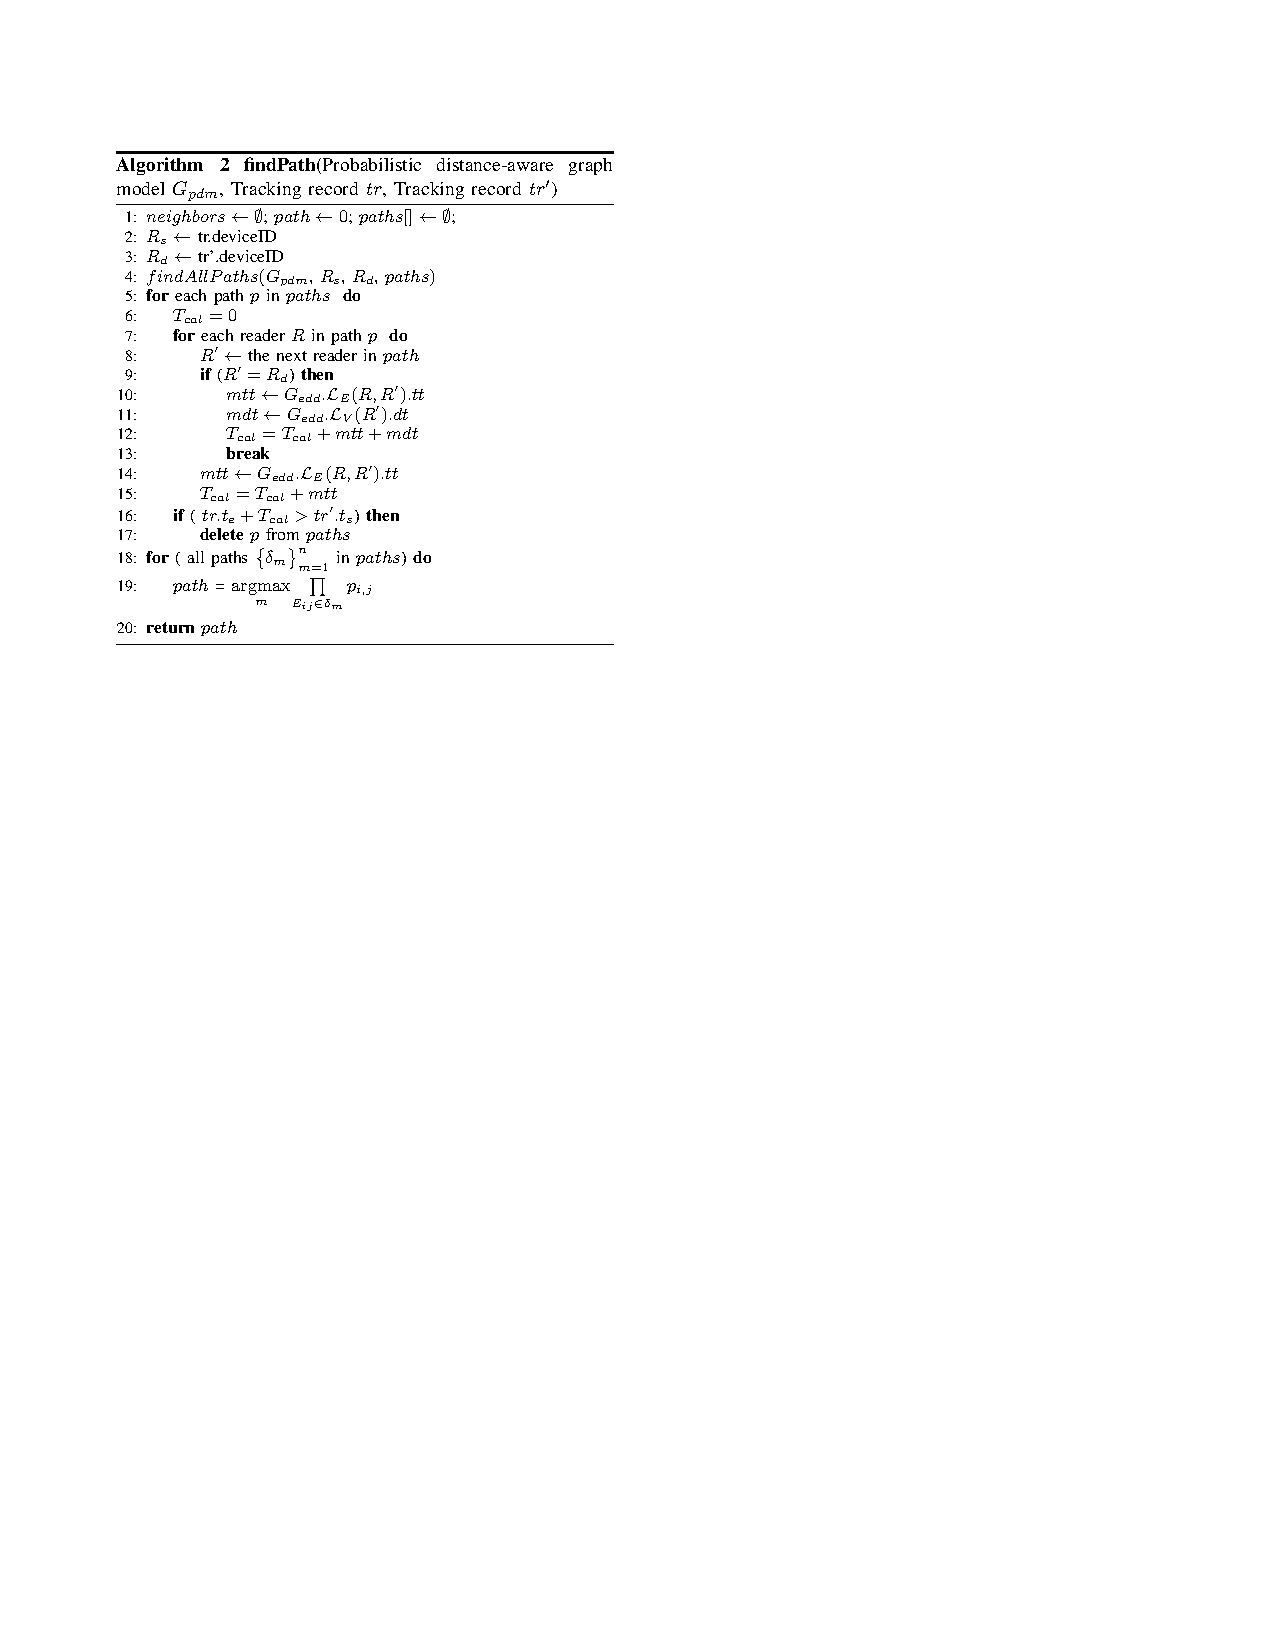
\includegraphics[width=\columnwidth]{figures/3-3/3-3-8.pdf}
  \end{figure}

  \column{0.5\textwidth}
  \begin{sitemize}
    \item takes graph model $G_{pdm}$ and two tracking records $tr$, $tr'$ as input.
    \item calls \emph{findAllPaths} to get all the possible paths between $R_s$ and $R_d$.
    \item lines 5-15: to check if the path satisfies the temporal constraint, a total traverse time ($T_{cal}$) is calculated, which is a time a moving object takes to traverse a path from $R_s$ to $R_d$.
    \item lines 17: if $T_{cal}$ is larger than the time object was first tracked the $R_d$, the path is treated as invalid and is deleted from the candidate paths.
    \item line 20: a most likely path is then estimated based on the maximum likelihood decision rule by using transition probabilities.
  \end{sitemize}

\end{columns}

\end{frame}


%------------------------------------------------

\begin{frame}
\frametitle{Recovering False Negatives}

\begin{itemize}

  \item retrieve a path between source reader $R_s$(tr.deviceID) and destination reader $R_d$(tr'.deviceID) in the graph and fills the missing readings of each reader a path contains between $R_s$ and $R_d$.

  \item the path retrieved is the most likely path, in a set of paths which satisfy the spatio-temporal constraints of subgraph between $R_s$ and $R_d$.

  \item to fill the missing readings, the parameters like, minimum travelling time between readers, minimum dwell time and sampling rate of corresponding reader are used.

  \item the approximate number of raw readings to be filled for each reader is determined as $\frac{\text{minimum dwell time}}{\text{sampling rate}}$.

\end{itemize}

\end{frame}

%------------------------------------------------

\begin{frame}
\frametitle{Conclusion}

This paper studies data cleansing for indoor RFID tracking data.\\~\\

It focuses one of the main aspects in raw indoor RFID tracking data, namely, \emph{false negatives}.\\~\\

A probabilistic distance-aware graph model is proposed to capture probabilities together with the spatio-temporal constraints implied by the deployment of RFID readers as well as indoor topology.\\~\\

The transition probabilities that capture likely an object move from one reader to another are obtained from the existing data.

\end{frame}
